\subsubsection{Buildings}
%Introduction
The emissions of the buildings sector is composed of stationary combustion and the construction of buildings. In 2018, it had an average contribution of 10.9\%
percent to the worlds greenhouse gas emissions. 
In this part, the goal was to make a monthly prediction of the 2020 emissions based on real time indicators that also were available long before the COVID-19 crisis in order to be able to correlate them.

%Materials and Methods
\paragraph{Indicators}

Sadly, the construction industry employment dataset was only updated until 2018, which is the reason why we chose to limit our datasets to the ones presented below:

\begin{itemize}
	\item \textbf{Producer price index by commodity for metals and metal producs: Iron Steel.}
	Source: Federal reserve Bank of St. Louis
	\url{https://fred.stlouisfed.org/series/WPU101}
	\item \textbf{Producer Price index by industry: cement and concrete product manufacturing.}
	Source:  Federal reserve Bank of St. Louis
	\url{https://fred.stlouisfed.org/series/PCU32733273}
	\item \textbf{Industrial Production: Durable Goods: Cement and concrete products.}
	Source:  Federal reserve Bank of St. Louis
	\url{https://fred.stlouisfed.org/series/IPG3273S}
	\item \textbf{Total construction spending.}
	Source:  Federal reserve Bank of St. Louis
	\url{https://fred.stlouisfed.org/series/TTLCONS}
\end{itemize}%todo: Were they all used? Spelling, Reduce info

The general idea was that the price should correlate with the demand for the product. Together with the assumption that the construction industry consumes a significant amount of the worlds concrete and steel production, the hypothesis is that we can use the prices as indicators in a machine learning model that is able to predict the emissions in 2020 based on previous price development.

In Figure \ref{fig:indicators}, selected indicators are plotted against the global \co emissions.
\begin{figure}[h!]
\centering
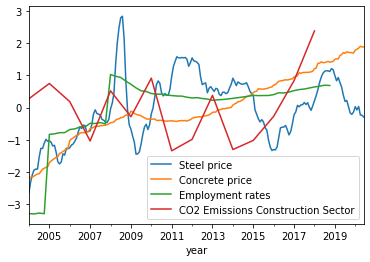
\includegraphics[width=0.4\linewidth]{../buildings/indicators}
\caption{Indicators and global \co emissions in arbitrary units.}
\label{fig:indicators}
\end{figure}
In general, one can observe that a slight correlation can already be seen on the global scale. of course, different countries are impacted differently from the prices. 
%todo: describe the raw plotted indicators against CO2 emissions

\paragraph{Strategy}

Our strategy to make use of the indicators was as follows:
\begin{enumerate}
	\item \textbf{Model training:} For each country a support vector machine regression model was used, in order to allow the employment of different kernels. The eight selected regions (USA, EU, Brazil, Russia, Japan, China, India, Canada)  were fitted on 2004-2018 yearly \co emission data. To avoid overfitting, the validation loss was optimized on 30\% of the data by using a gridsearch method to evaluate the best degree of kernel regularization. 
	\item \textbf{Prediction:} Afterwards, the model was used to predict monthly data in 2020 with the same indicators.
	\item \textbf{Extracting COVID-19 influence:} To extract the information whether the emissions had gone down or not due to COVID-19, we compare the 2020 data with an interpolation of the global emissions up to 2018.
\end{enumerate}

%Results
\paragraph{Results}

First, the gridsearch with k fold cross validation was executed to retrieve the best regularization parameter and kernels to reduce overfitting.

For each country the gridsearch provided different optimal kernels and regularization strengths. The resulting parameters are provided in Table \ref{buildings:kernel} together with the resulting scores.

\begin{table}[h!]
	\centering
	\begin{tabular}{clll}
		\hline
		Country & Regularization strength & Kernel & negative RMS error \\
		\hline
		\hline 
		EU & 'C': 10 & 'rbf' &
		-0.67 \\
		United States & 'C': 10 & 'poly' & 
		-0.74 \\
		India &'C': 10 & 'poly' &
		-0.23 \\
		China &'C': 100 &  'rbf' &
		-0.36 \\
		Japan &  'C': 10 & 'rbf' &
		-0.32 \\
		Russia &'C': 10 & 'poly' &
		-0.67 \\
		Canada &'C': 10 & 'rbf' &
		-1.20 \\
		Brazil &'C': 10 & 'rbf' &
		-0.38 \\
		\hline 
		&&& \\
	\end{tabular}
	\caption{Resulting parameters.}
	\label{buildings:kernel}  
\end{table}



\begin{figure}[h]
	\centering
	\subfloat[EU]{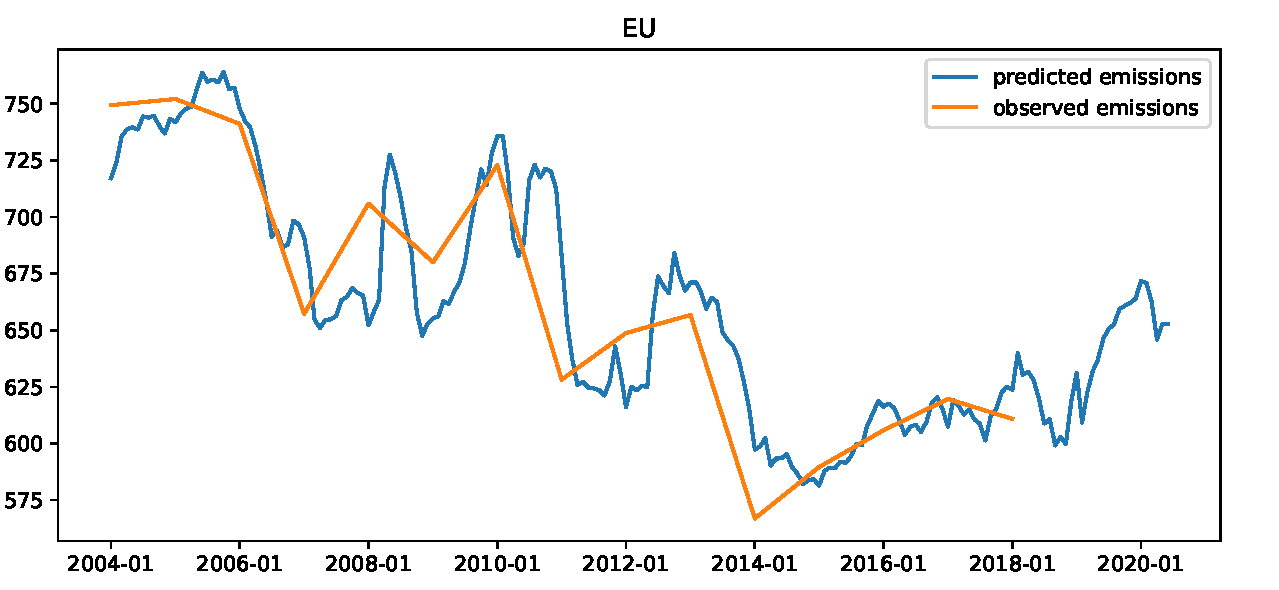
\includegraphics[width=0.5\linewidth]{../buildings/eu}}
	\subfloat[USA]{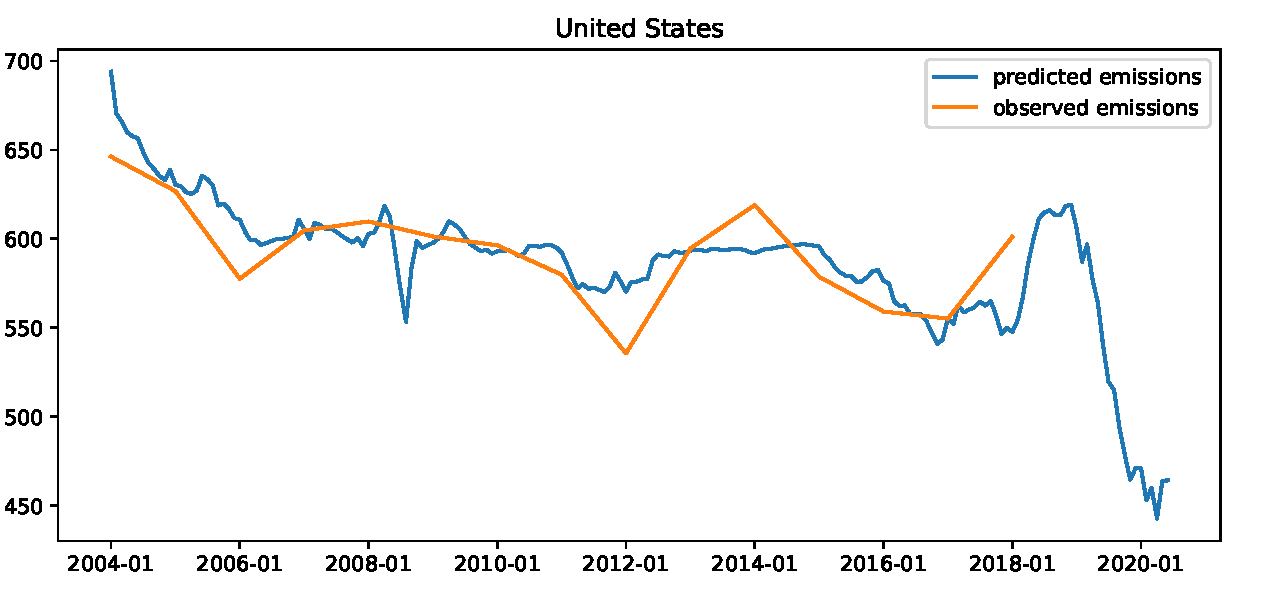
\includegraphics[width=0.5\linewidth]{../buildings/united_states}}\\
	\subfloat[Brazil]{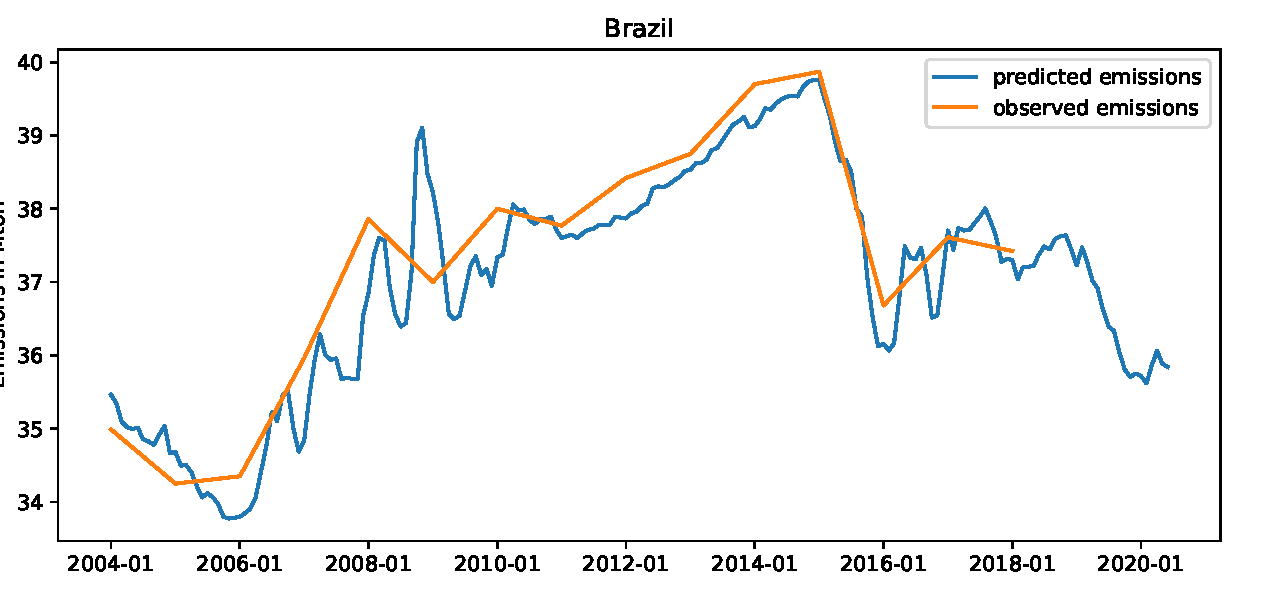
\includegraphics[width=0.5\linewidth]{../buildings/brazil}}
	\subfloat[Russia]{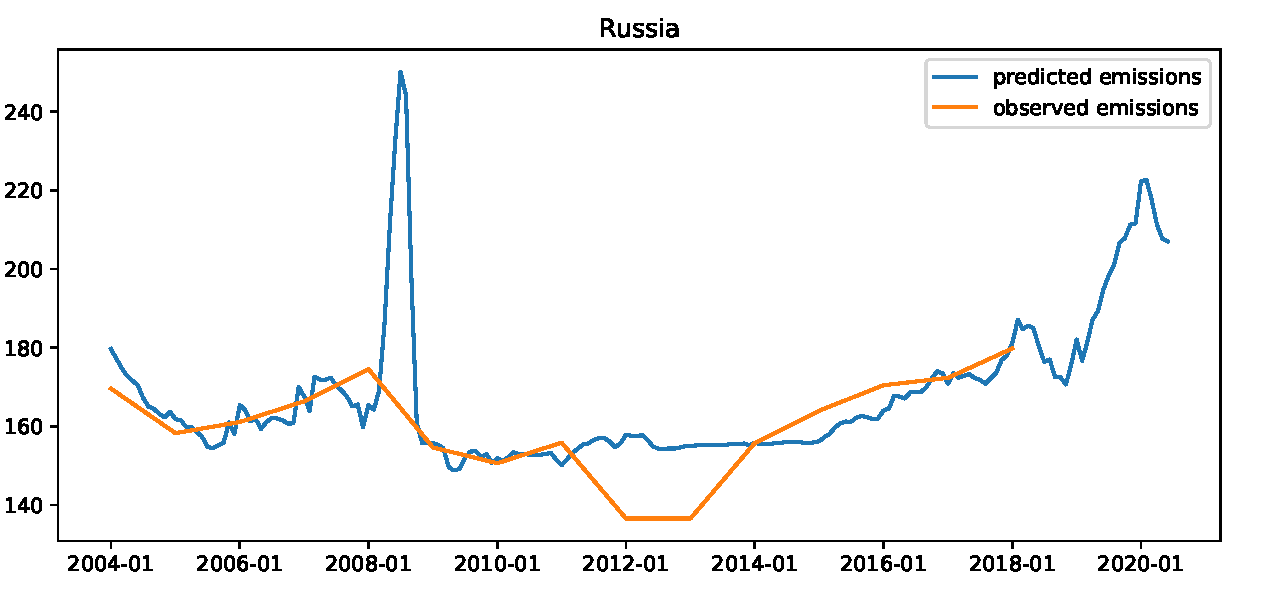
\includegraphics[width=0.5\linewidth]{../buildings/russia}}\\
	\subfloat[India]{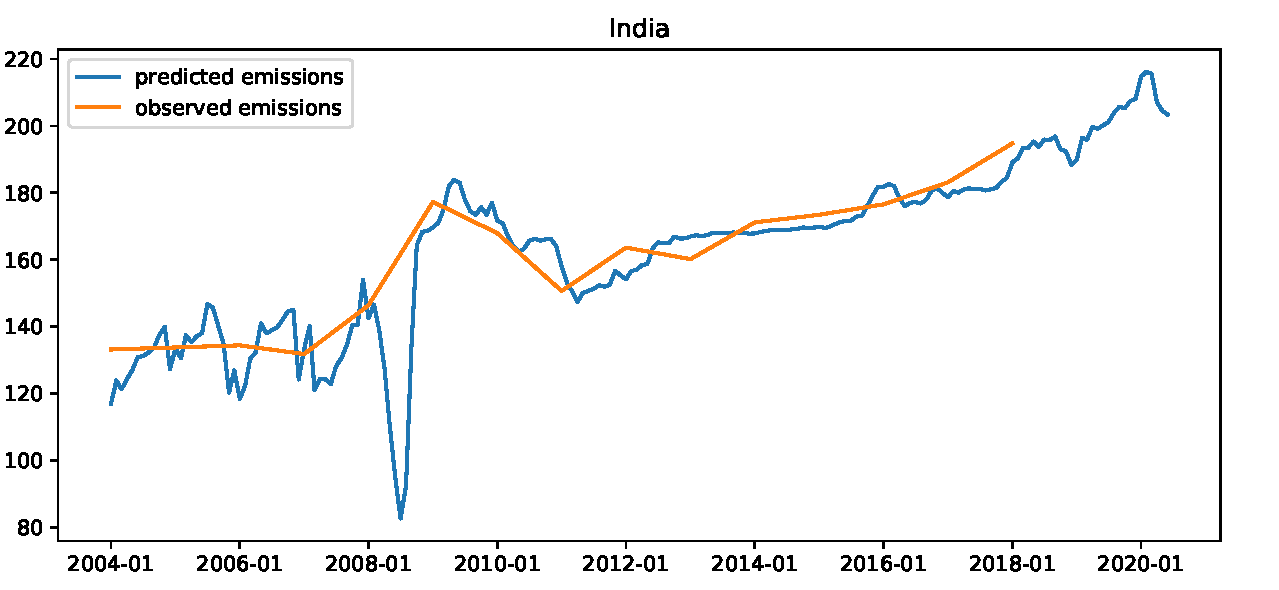
\includegraphics[width=0.5\linewidth]{../buildings/india}}
	\subfloat[Japan]{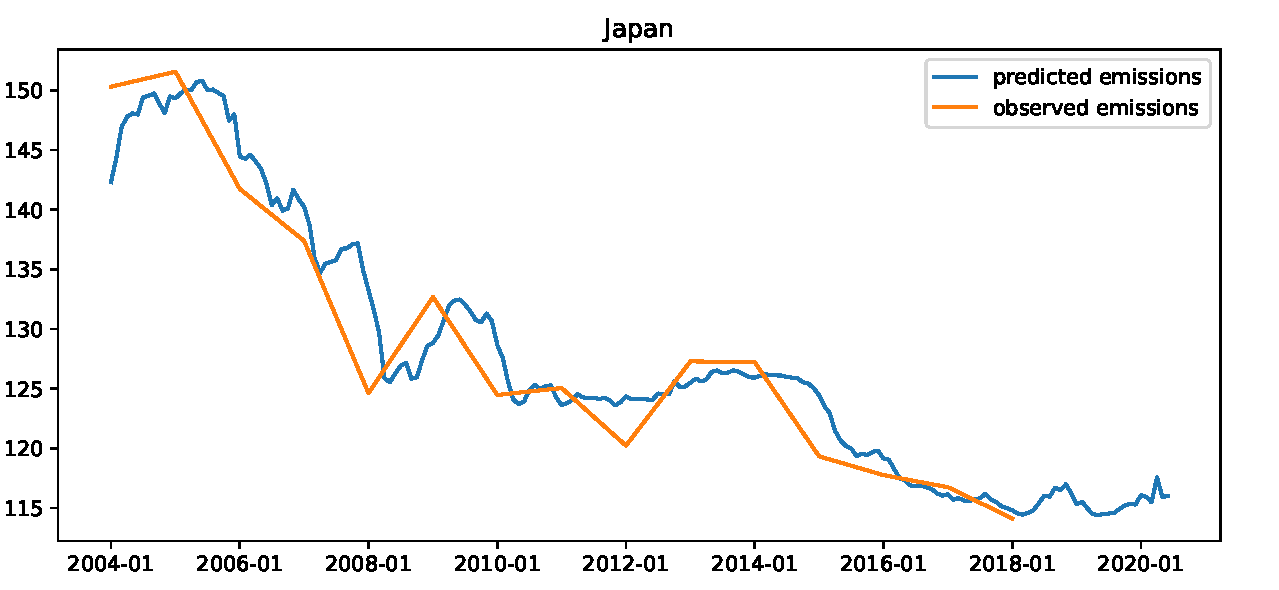
\includegraphics[width=0.5\linewidth]{../buildings/japan}}\\
	\subfloat[Canada]{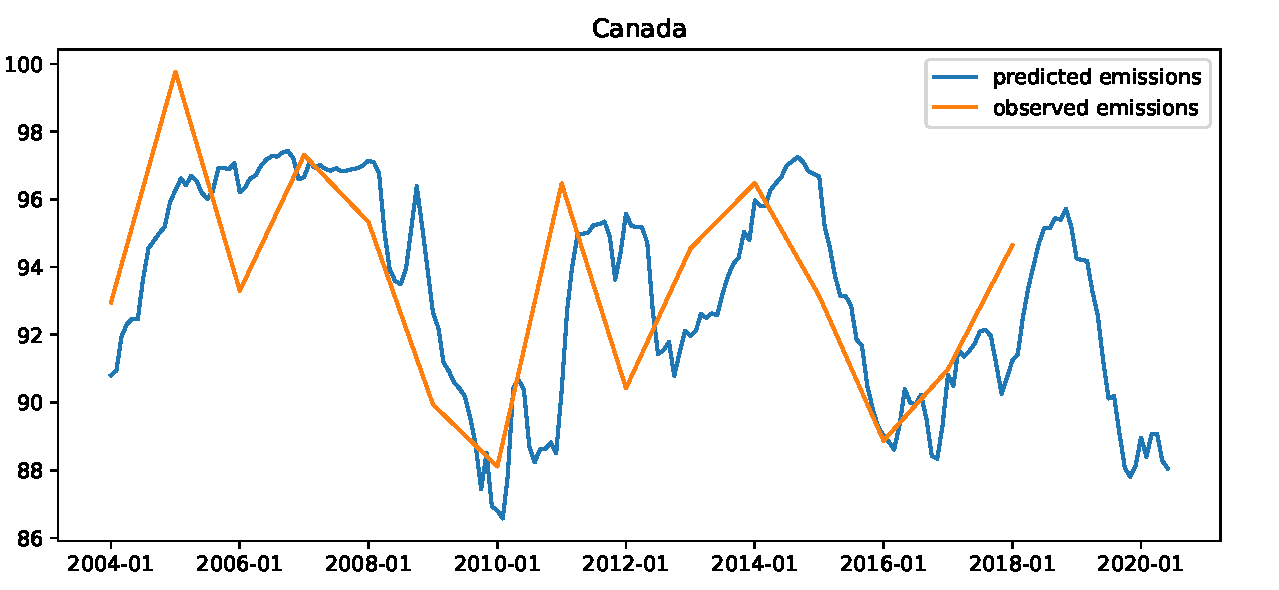
\includegraphics[width=0.5\linewidth]{../buildings/canada}}
	\subfloat[China]{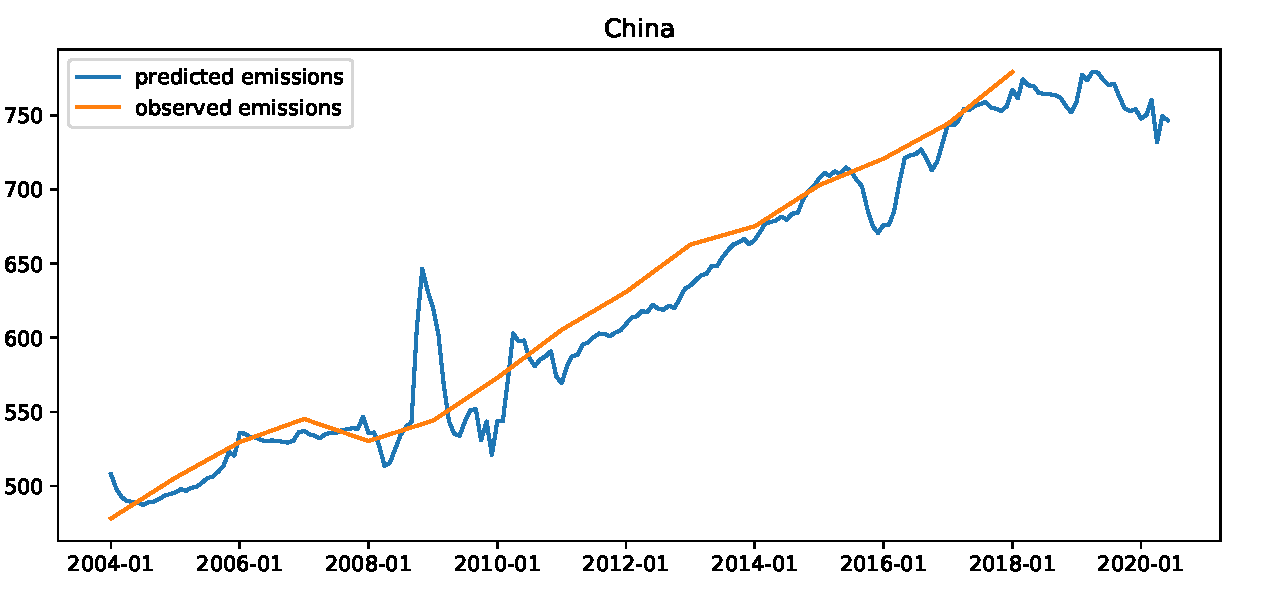
\includegraphics[width=0.5\linewidth]{../buildings/china}}
	\caption{Predicted emissions based on indicators on training set and for 2020.}
	\label{fig:mobility_pred}
\end{figure}	


%Conclusion
\paragraph{Conclusion}

In conclusion, we were able to model the countries sufficiently well. Each country showed an emission drop in the early months of 2020, indicating that COVID-19 had an impact on the indicators and therefore on the overall emissions in the sector.
%todo: scores are lacking